% !TeX spellcheck = fr_FR
\chapter{Les \Jiben{} \Jianfa{}}\label{ch:jibenjianfa}

Le terme  \Jiben{} \Jianfa{} (\begin{CJK*}{UTF8}{bsmi}基本劍法\end{CJK*}) désigne ce qu'on appelle généralement les techniques de base de l'épée. On peut le traduire mot à mot par : les \textit{méthodes} (\Fa{}) \textit{basiques}, \textit{élémentaires}, \textit{fondamentales} (\Jiben{}) de l'\textit{épée droite} (\Jian{}).

Les différents styles de \Taijijian{} présentent un nombre variable de \Jiben{} \Jianfa{}, habituellement entre quatre et treize ou même plus. On trouve déjà le nom de plusieurs de ces techniques dans le \JianJing{}, un traité d'épée écrit par \YuDayou{} aux environs de 1560, ou dans le \WubeiZhi{}, une encyclopédie militaire qui aurait été publiée en 1620.
Il n'est pas certain cependant que ces termes se rapportaient déjà aux techniques qu'ils décrivent aujourd'hui en \Taijijian{}, d'autant moins que les noms des \Jiben{} \Jianfa{} sont loin de toujours se correspondre d'un style à l'autre.

La tradition du \Yangjia{} \Michuan{} \Taijijian{} énumère huit \Jiben{} \Jianfa{}, chacun correspondant à une des huit sections de la forme d'épée \Kunlun{} : \Pi{}, \Ci{}, \Liao{}, \Zha{}, \Mo{}, \Duo{}, \Tiao{}, \Hua{}.
Un neuvième, \Dian{}, est aussi mentionné mais est parfois décrit comme la combinaison de \Pi{} et \Ci{}, peut-être pour préserver le nombre parfait de huit techniques pures.
Quelle qu'en soit la raison, j'ai le sentiment que cette description de \Dian{} en tant que combinaison, constitue un aveu de la possibilité d'associer les \Jiben{} \Jianfa{} entre eux.
Je préfère donc les considérer, non pas comme des techniques en soi, mais plutôt comme des principes techniques qu'on peut combiner pour générer l'ensemble des techniques possibles. Ce qu'on appelle alors \textit{techniques de base} seraient ainsi simplement les techniques représentatives des \Jiben{} \Jianfa{} qui les constituent.

L'examen des caractères chinois pour les huit \Jianfa{} du \Yangjia{} \Michuan{}, révèle que quatre d'entre eux (\Pi{} \begin{CJK*}{UTF8}{bsmi}劈\end{CJK*}, \Ci{} \begin{CJK*}{UTF8}{bsmi}刺\end{CJK*}, \Duo{} \begin{CJK*}{UTF8}{bsmi}剁\end{CJK*}, \Hua{} \begin{CJK*}{UTF8}{bsmi}劃\end{CJK*}) possèdent la clé graphique du couteau, tandis que les autres (\Liao{} \begin{CJK*}{UTF8}{bsmi}撩\end{CJK*}, \Zha{} \begin{CJK*}{UTF8}{bsmi}扎\end{CJK*}, \Mo{} \begin{CJK*}{UTF8}{bsmi}抹\end{CJK*}, \Tiao{} \begin{CJK*}{UTF8}{bsmi}挑\end{CJK*}) contiennent la clé de la main. On peut donc avancer que les quatre premiers précisent principalement la manière dont la lame est utilisée pour couper ou percer tandis que les autres décrivent plutôt le mouvement général (soulever, fouetter, etc.) indépendamment de l'arme. On trouve par exemple les caractères \Liao{} et \Zha{} dans le nom de techniques de lance, de bâton ou même de boxe, citées dans divers manuels d'arts martiaux historiques. La neuvième technique, \Dian{} \begin{CJK*}{UTF8}{bsmi}點\end{CJK*}, dont le nom signifie \textit{pointer}, est encore une exception puisqu'elle ne contient aucune des deux clés graphiques et ainsi, mettrait l'accent sur l'utilisation de la pointe de la lame.

Les descriptions des \Jiben{} \Jianfa{} du \Yangjia{} \Michuan{} \Taijijian{} ne seront pas présentées ci-dessous dans leur ordre traditionnel, suivant la suite des sections correspondantes de la forme d'épée \Kunlun{}. Au lieu de cela, je présenterai dans un premier temps les quatre techniques de lame avant de passer aux autres. Ce sont là des interprétations personnelles prenant en compte le point de vue exposé plus haut et s'appuyant sur les enseignements de Maître Wang ainsi que sur des textes historiques. Le contenu de ce chapitre, bien qu'étant centré sur la tradition du \Yangjia{} \Michuan{}, devrait toutefois être plus largement applicable, au moins en partie, aux autres styles.

% !TeX spellcheck = fr_FR
\section{\Pi{}}
En chinois, \Pi{} \begin{CJK*}{UTF8}{bsmi}劈\end{CJK*} signifie \textit{couper}, \textit{fendre}, \textit{aller droit vers}. En substance, \Pi{} est une coupe fendante.

En tant que technique de base, \Pi{} est simplement décrit comme une coupe verticale descendante. Elle est souvent associée à un moulinet intérieur ou extérieur que je ne décrirai pas ici puisqu'il ne fait pas strictement partie de la technique \Pi{} et aura plutôt sa place ailleurs.

Bien que la technique formelle \Pi{} soit dirigée vers le bas, je pense personnellement que l'énergie fendante de \Pi{} peut être orientée dans toute direction. Ainsi, même des coupes horizontales ou montantes qui fendent la cible de manière caractéristique sans aucun mouvement de trancher peuvent être en quelque sorte considérées comme affiliées à cette énergie.

La technique emblématique formelle \Pi{} se prépare en levant la poignée de l'épée à hauteur d'oreille pendant que l'on s'assied dans la jambe opposée à la main armée. La prise doit être relâchée mais fermement maintenue entre le majeur, l'annulaire et le pouce. Le contact relâché des autres doigts maintient un contrôle de la poignée tout en permettant une certaine flexibilité de la prise.
Dans un contexte moins formel et moins statique, on peut combiner cette préparation à un déplacement pendant une parade ou une esquive, dans une transformation continue de l'action défensive en riposte.

Dans la première phase de la coupe, la main est envoyée en diagonale et tire l'épée en avant vers le bas dans la direction du pommeau pour accélérer la lame. La force de biais exercée par la main sur la poignée entraîne ainsi graduellement la rotation de l'épée autour de son centre de gravité (fig. \ref{fig:pi_cut} a).

Ce mouvement tire son énergie de l'expansion du corps et le cas échéant d'un pas vers l'avant pour une portée plus importante et un gain de puissance.

Ensuite, dès que le centre de gravité a passé en avant de la main (fig. \ref{fig:pi_cut} b), celle-ci cesse d'exercer toute action et ne fait plus que suivre la poignée en maintenant simplement un contrôle relâché mais ferme de la trajectoire de l'épée. La lame se déplace ainsi librement avec une trajectoire non perturbée au moment où elle atteint la cible et toute l'énergie cinétique accumulée lors de la phase d'accélération est alors transférée dans la coupe (fig. \ref{fig:pi_cut} c).

\begin{figure}[ht]
\centering
	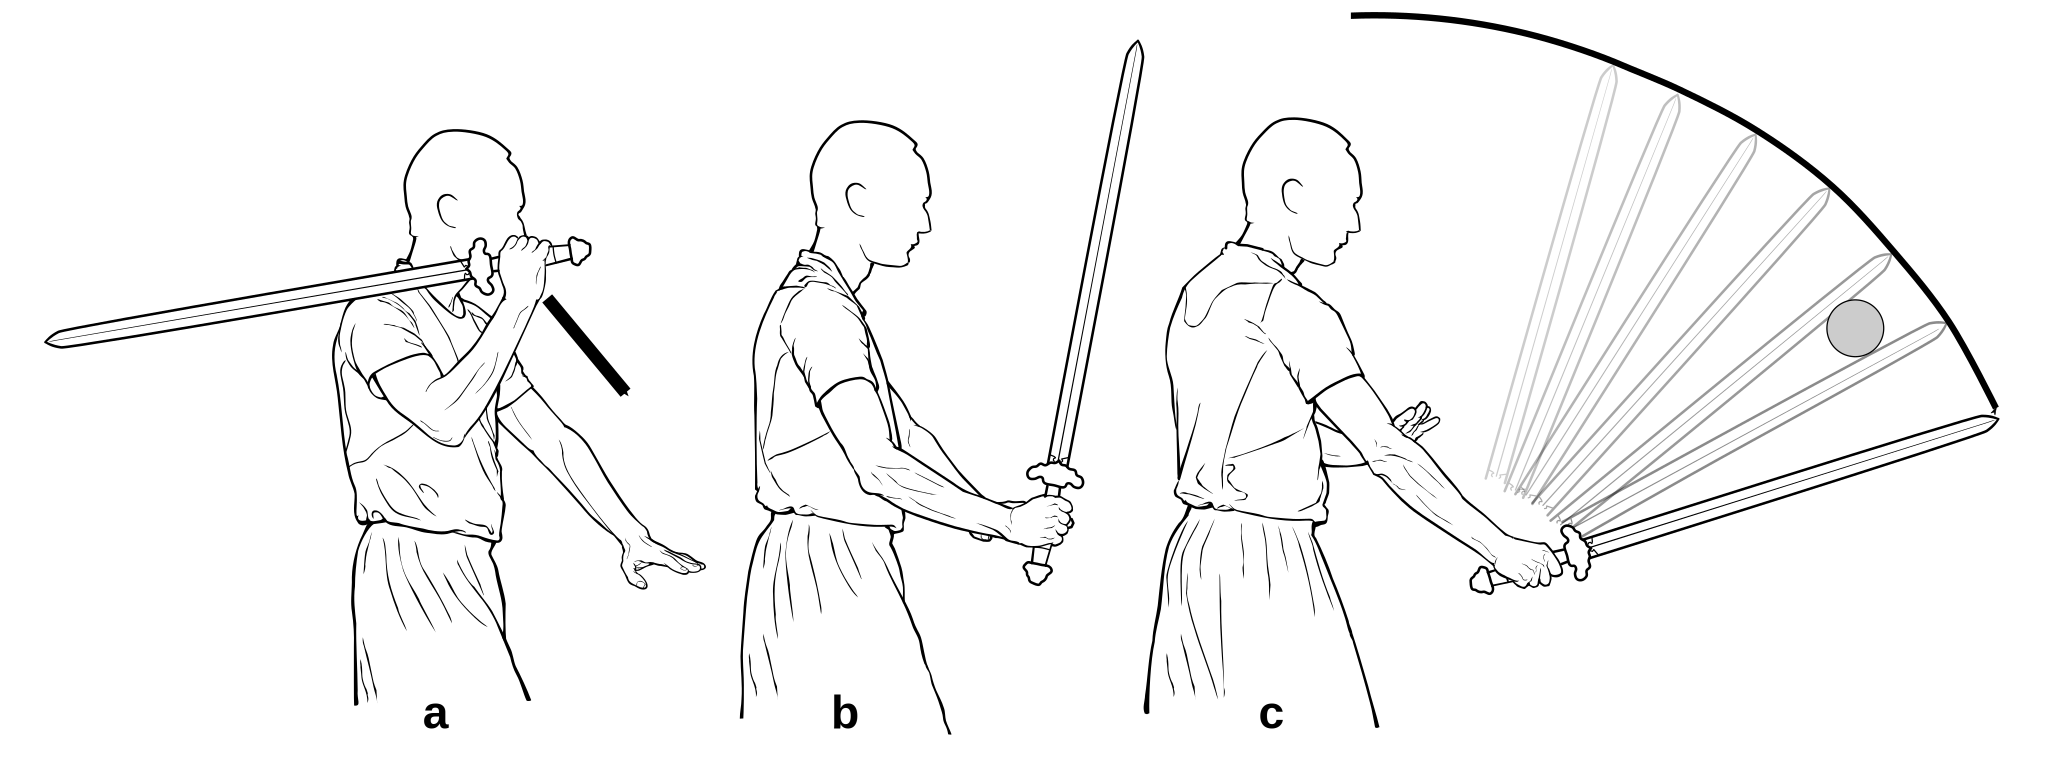
\includegraphics[width=1.00\textwidth]{../../Images/JibenJianfa/Pi/Pi_juxtaposed.pdf}
	\caption[Coupe \Pi{}]{Coupe \Pi{} : (a) Partant d'une position haute de l'épée, la main droite la tire vers le bas pour accélérer la lame; (b) montre la fin de la phase d'accélération, à partir de cet instant, la main n'exercera plus d'action sur la poignée; (c) la main suit la poignée avec juste un contrôle ferme de la trajectoire de l'épée de manière à ce que la lame puisse librement traverser la cible représentée par un cercle gris. Notez que la trajectoire de la pointe n'est pas un cercle mais un arc allongé.}
	\label{fig:pi_cut}
\end{figure}

Il est absolument indispensable que le plat de la lame soit parfaitement aligné avec la trajectoire de la l'épée pour garantir que le poids de la lame soit derrière le tranchant pour le pousser à travers la cible. Si jamais la lame atteignait la cible avec un angle, aussi petit soit-il, elle tendrait à tourner autour de son axe et pourrait rebondir dangereusement au lieu de trancher. Lorsque l'alignement est correct, au contraire, et que la prise est relâchée, la lame pourra traverser la cible de part en part sans retour notable.

Après la coupe, la poignée bute naturellement contre le talon de la main et les doigts resserrent leur prise pour arrêter l'épée dans une position de garde à hauteur de taille, sans aucune tension ni rebond. Grâce à une bonne structure corporelle, l'énergie de l'épée retourne ainsi au corps, aidant le recentrage, et la préparation de la technique suivante.
% !TeX spellcheck = fr_FR
\section{\Hua}
Le verbe \Hua{} \begin{CJK*}{UTF8}{bsmi}劃\end{CJK*} signifie \textit{délimiter}, \textit{tracer}. Ce caractère est aussi une variante du mot désignant un trait dans un caractère chinois.
La partie de gauche de ce caractère étant la clé du pinceau, ces observation suggèrent que cette technique évoque la notion de calligraphie, d'écriture et de dessin.

Le \Yangjia{} \Michuan{} présente la technique \Hua{} emblématique comme une coupe horizontale ou un large mouvement horizontal dans le but de maintenir les adversaires à distance. L'idée est ici de balayer l'espace avec l'épée pour délimiter la zone la plus large possible autour de soi et d'entailler quiconque ose s'approcher.

D'une manière plus générale, les coupes \Hua{} ne sont pas systématiquement horizontales et s'appliquent à différentes distances, depuis des entailles réalisées à longue distance avec la pointe de l'épée, jusqu'à des coupes glissées avec toute la longueur du tranchant à courte distance. Dans tous les cas, les coupes \Hua{} ont pour caractéristique commune le fait que la lame trace progressivement une longue entaille, au contraire de \Pi{} qui fend la cible d'un coup. 

Pour réaliser une coupe \Hua{} à longue distance, l'épée est lancée en avant et, lorsque le bras a presque atteint son extension complète, juste avant que la lame ne frappe la cible, la prise se resserre doucement sur la poignée pour assurer la connexion entre les centres de l'épée et du corps. La rotation continue ainsi à partir de l'épaule tandis que l'épée tire le corps en avant jusqu'à ce que la portée maximale soit atteinte (fig. \ref{fig:hua_cut} a-c). Ensuite, la prise agissant comme un levier, l'inertie de l'épée repousse la poignée contre le talon de la main, engendrant un mouvement vers l'arrière qui génère une coupe glissée et recentre le corps dans une posture de garde (fig. \ref{fig:hua_cut} d-f). 

\begin{figure}[ht]
\centering
	\includegraphics[width=1.00\textwidth]{../../Images/JibenJianfa/Hua/Hua.pdf}
	\caption[Coupe \Hua{}]{Coupe \Hua{} : (a) \'{A} partir d'une position haute de l'épée, (b) la main droite lance le pommeau vers l'avant; (c) montre la fin de la phase active de la technique; (d) à (f) pendant la phase passive, l'inertie de l'épée repousse la main en arrière, réalisant la coupe glissée et recentrant le corps en position.}
	\label{fig:hua_cut}
\end{figure}

\'{A} plus courte distance, la dynamique des coupes \Hua{} utilise moins l'inertie de l'épée mais s'appuie plus sur la structure et le mouvement du corps. Dès que le tranchant est en contact, la coupe est effectuée en pressant le tranchant contre la cible et en tirant l'épée selon une direction parallèle à l'épée, en se déplaçant ou en tournant le corps. Il est parfois possible, en particulier en passant dans le dos de l'adversaire, de réaliser avec le faux tranchant une coupe \Hua{} à courte distance.

En plus d'être une coupe glissée, \Hua{} peut aussi être utilisé pour maintenir des adversaires à distance ou les obliger à réagir de façon à exploiter leur action et prendre le contrôle du rythme. Pour ce faire, on peut lancer une coupe \Hua{} sans toutefois s'engager totalement, ou faire des moulinets tout en avançant. La distance doit dans ce cas est suffisamment courte pour que ces coupes soient clairement perçues comme une menace bien qu'on puisse être légèrement hors de mesure. La distance idéale est à la limite supérieure de la mesure courte, distance à laquelle, bien qu'elle soit incertaine, une touche est tout à fait plausible et l'adversaire ne peut que se sentir obligé de réagir défensivement. Il est important dans ce cas de se préparer à doubler avec une attaque plus engagée ou un contrôle de la lame selon les circonstances. C'est cette seconde intention qui permettra de prendre l'initiative en exploitant l'action de l'adversaire.

En rompant la distance après une attaque infructueuse, il est possible de maintenir l'adversaire à distance avec une série de moulinets que Maître Wang Yennien décrivait également comme étant des coupes \Hua{}. Cette application de la technique correspond parfaitement à la traduction \textit{délimiter} puisqu'elle crée en effet une zone de sécurité empêchant l'adversaire d'entrer et d'attaquer pendant qu'on se place hors de mesure.

% !TeX spellcheck = fr_FR
\section{\Ci{}}
On trouve le mot \Ci{} \begin{CJK*}{UTF8}{bsmi}刺\end{CJK*}, signifiant \textit{estoquer}, \textit{percer}, \textit{poignarder}, dans le \WubeiZhi{} comme terme générique désignant l'ensemble des techniques d'estoc à l'épée. D'autres traités anciens le mentionnent aussi pour décrire les estocs avec diverses armes. 

Dans la tradition du \Yangjia{} \Michuan{}, \Ci{} est défini comme un estoc horizontal ou remontant, poussant la pointe puissamment à travers la cible. 

On réalise généralement la technique formelle en commençant sur le pied droit, pied gauche en avant, soit avec une passe avant (\Ci{} long), soit avec un simple transfert de poids sur le pied gauche (\Ci{} court). Dans le contexte formel des exercices et de la forme, la cible du \Ci{} court est l'abdomen, celle du long est la base de la gorge. En assaut par contre, on peut viser d'autres cibles telles que le torse, ou même le visage.

Que la technique réalisée soit longue ou courte, on commence invariablement par créer dans le corps une structure spiralée connectant le pied gauche et l'épée. Dès que la taille bouge, le bras droit pousse sur la poignée et se lève en un mouvement spiralé qui s'achèvera avec une position d'épée horizontale, sur son plat, le pommeau orienté vers la hanche gauche. Dans le même temps, on transfère le poids sur le pied gauche. La prise de l'épée s'adapte progressivement pour maintenir une connexion ininterrompue entre la main et la poignée, sans aucun angle, permettant de pousser sans effort l'épée vers avant. Cet ajustement permet également d'exercer sur la poignée une action oblique atteignant au delà de la garde le point générant un point pivot dans la pointe de la lame pour la stabiliser\footnote{Voyez le chapitre \ref*{ch:epeechinoise} pour de plus amples détails sur les points pivots.}. 


La passe avant du \Ci{} long permet une portée plus longue. Le bras droit doit être étendu avant d'avancer pour augmenter la précision de l'estoc et placer le corps derrière l'épée, aussi loin que possible du danger. Engager la lame de l'adversaire pour la contrôler avec la garde ou le fort de la lame, permet encore une meilleure protection. 

\begin{figure}[ht]
\centering
	\includegraphics[width=1.00\textwidth]{../../Images/JibenJianfa/Ci/Ci_thrust_arc.pdf}
	\caption[Estoc \Ci{} long]{\`{A} la fin de l'estoc \Ci{} long, l'épée est alignée avec la hanche gauche mais sa pointe est dirigée vers le centre, visant la base de la gorge. La puissance de toute la structure du corps se concentre dans l'épée pour pousser la pointe à travers la cible.}
	\label{fig:ci_thrust}
\end{figure}

Idéalement, le talon droit devrait toucher le sol exactement au moment où la pointe de la lame atteint la cible. Le relâchement de la structure achève alors le pas en poussant la lame au travers de la cible. Il est important de ne pas se laisser tomber dans la jambe droite de manière à conserver une capacité de se retirer rapidement en cas de nécessité. Cela ne signifie toutefois pas qu'on ne doit jamais transférer le poids sur la jambe droite, mais que la polarité vide/plein entre les deux jambes doit être maintenue en toutes circonstances pour éviter la double lourdeur. L'arc de force venant du pied gauche, traversant le dos, spiralant le long du bras droit jusqu'à la pointe de l'épée, et soutenu par la spirale du bras gauche, génère ainsi une structure à la fois puissante et mobile.

% !TeX spellcheck = en_GB
\section{\Duo}
The translation of \Duo{} \begin{CJK*}{UTF8}{bsmi}剁\end{CJK*}, referring to the cooking term \textit{to mince}, somehow suggests repetition and cutting using a part of the blade further away from the tip than \Pi{}. The movement itself is a combination of a forward extension with some sort of shearing, as if using a large cooking knife to mince herbs or vegetables.

In the \Yangjia{} \Michuan{} tradition, the emblematic \Duo{} is performed with both arms extended almost in line with the sword's blade (fig. \ref{fig:duo_full}). 


\begin{figure}[ht]
	\centering
	
	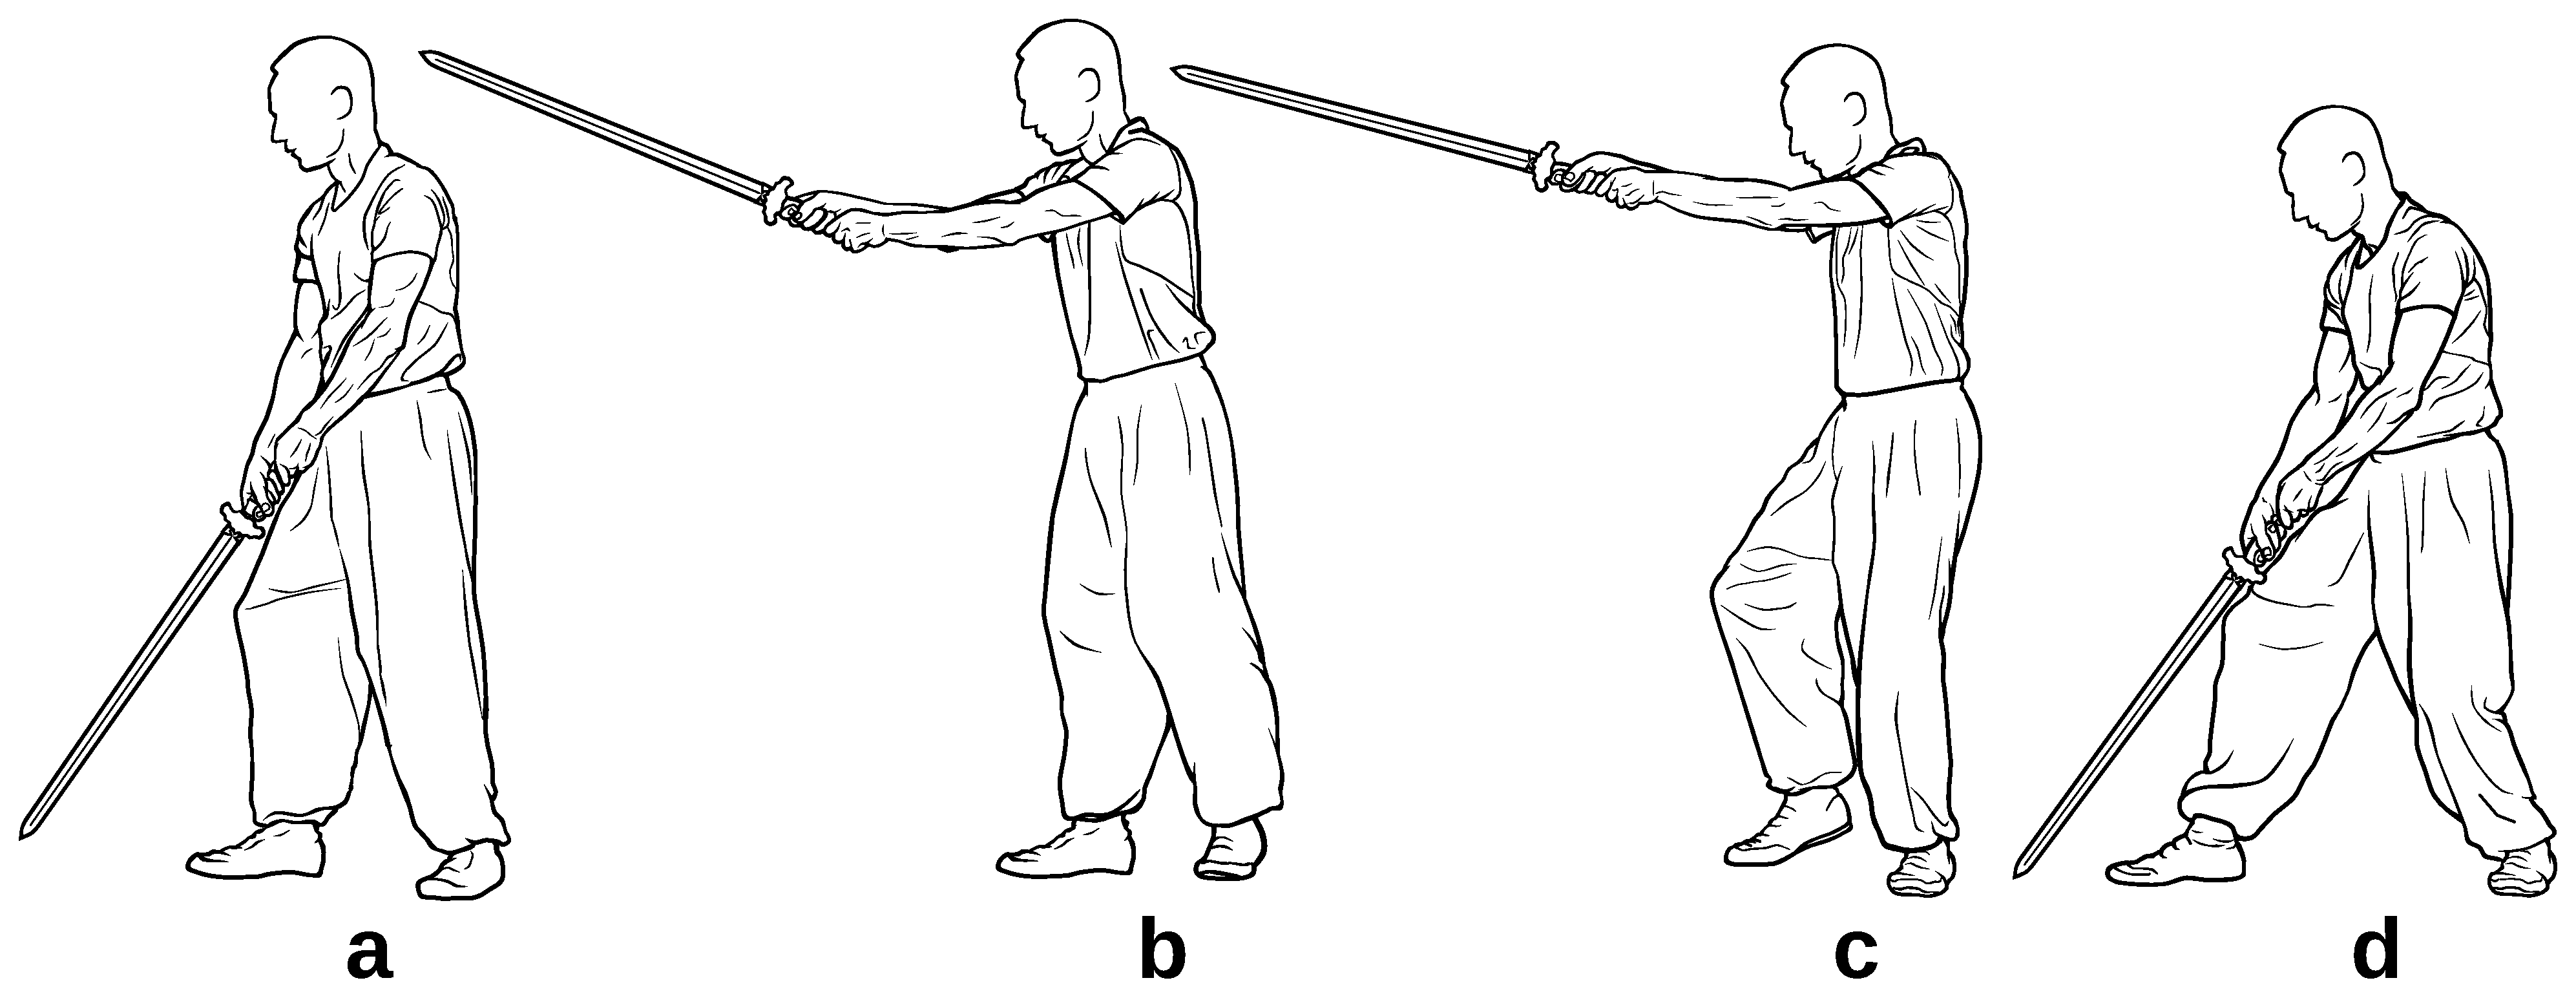
\includegraphics[width=1.00\textwidth]{../../Images/JibenJianfa/Duo/Duo.pdf}
	\caption[Advancing \Duo{}]{\Duo{} in the forward direction. From a low guard (a), raise the sword with a transfer of the weight onto the right foot (b), invert polarity and transfer the weight back onto the left foot (c), drop the sword while sinking in the left leg and advancing the right foot.}
	\label{fig:duo_full}
\end{figure} 

Even though both hands are in contact with the handle,  this should not be mistaken for a true double handed grip of the sword. While raising the sword and advancing, the right hand holds the sword while the left hand provides the structure and power coming from the waist by acting on the pommel along the direction of the blade. The combination of the right hand's passive role with the left hand's action creates a polarity resulting in a movement of the sword perpendicular to the axis of the right arm. When lowering the sword, the roles of both hands are inverted (fig. \ref{fig:duo_detail}). 

\begin{figure}[ht]
	\centering
	
	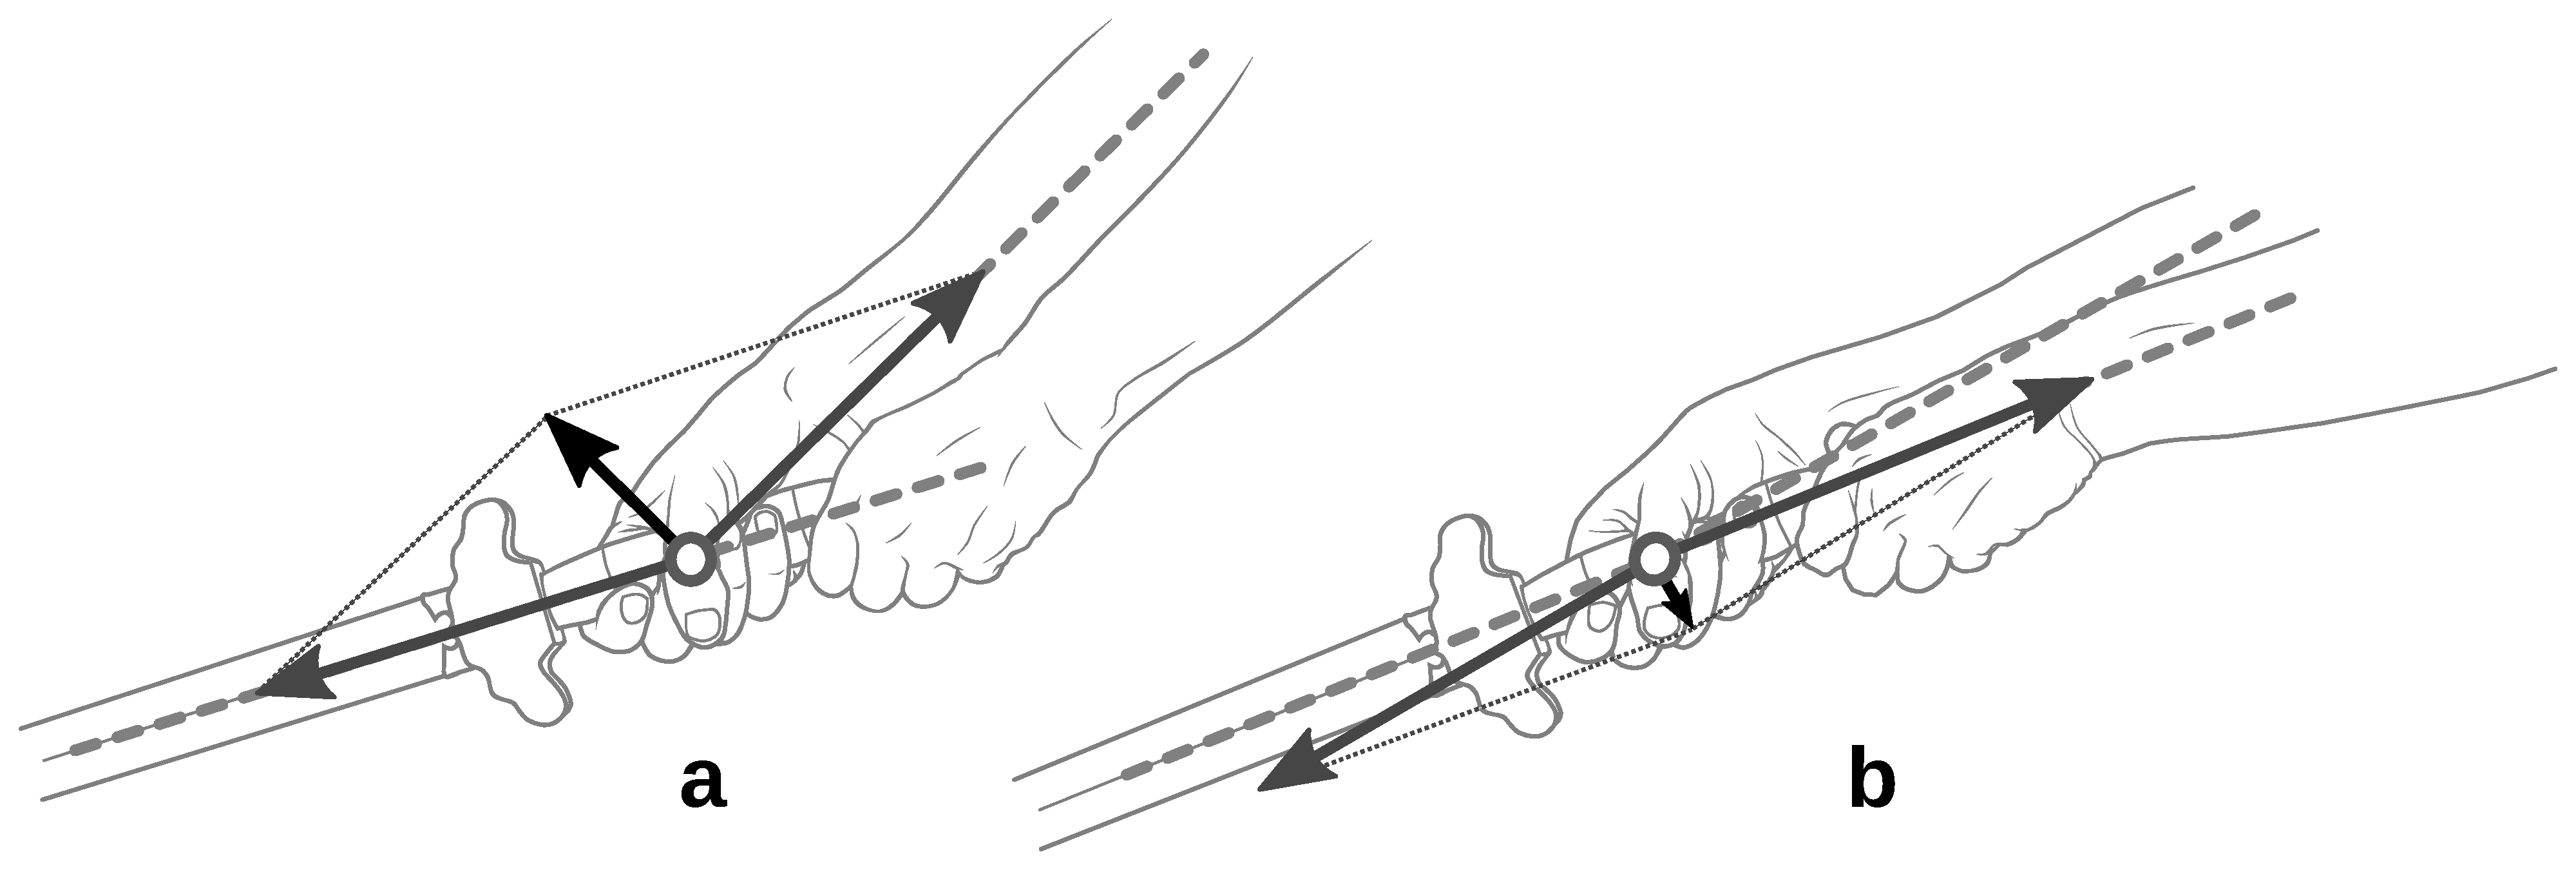
\includegraphics[width=1.00\textwidth]{../../Images/JibenJianfa/Duo/DuoDetail.pdf}
	\caption[Balance of forces in \Duo{}]{(a) To perform a forward rising \Duo{}, the left hand pushes the handle in the direction of the blade tip while the right arm passively balances the pushing force. Due to the angle between the pushing direction and the right arm, the resulting force perpendicular to the right arm pushes the sword upwards.\\
	(b) To perform a forward descending \Duo{}, the right hand pushes the handle while the left arm passively balances this force. The resulting force perpendicular to the left arm, draws the sword downwards.
	}
	\label{fig:duo_detail}
\end{figure} 

The power of the ascending forward \Duo{} thus originates in the weight transfer from the rear leg onto the fore leg, is transmitted to the sword by the left/rear hand with the right/fore hand exactly and passively balancing the forces to effortlessly generate the technique. An effective connexion between the waist and the sword will allow the explosive expression of the \Duo{} technique. 
This method somehow echoes the precepts found in the \JianJing{} stating that, when wielding a double-handed sword, power is first in the waist, then in the rear hand, and finally in the fore hand.

For the retreating \Duo{}, however, the hands play a reversed role: the right hand is active when raising the sword, and passive otherwise. As a rule of thumb, advancing or retreating, the active hand is always the one on the same side as the foot that is moving.

Since, when cooking, herbs are usually minced by cutting downwards, we may argue that the active phase of \Duo{} is the descending one. However, if we examine attentively the actual movement of a kitchen knife when mincing, we may discover that its form when cutting actually corresponds to the rising phase of \Duo{}. The main difference is that the tip of the knife stays down in contact with the table whereas the point of the sword rises up. But, in both cases, the edge follows the same movement relative to the tip. 
However, it is perfectly possible to be active in both phases, the actual passive phase being the transition movement between the ascending and descending parts of the technique. Thus, \Duo{} can be a raising thrust or cut as well as a descending cut, or, combined with \Mo{} energy, an action on the opponent's blade, either ascending to intercept and deflect or descending to shear. 

It is worth noting at this point that, since both hands are in contact with the hilt, the sword is always in line with the axis of the body. This axis is more to the left when we are on our left foot, in the low on-guard position that precedes the ascending forward phase of \Duo{}. Then, during the lifting phase of the movement, the axis is shifting to the right before being transferred back to the left when descending. Therefore, in the deflect/shear application of  \Duo{} in combination with \Mo{}, during the upward interception/deflection, transferring the weight onto the right/forward leg gently pushes the opponent's tip away, allowing the descending shear to naturally aim at the centre of the opponent's sword, deflecting it further to open the way for a hit while preventing any counter attack. 

\fiche{The simplest application of \Duo{} starts with a lower guard as an invitation for the opponent to prepare an attack. We can then engage and deflect with a \Duo{} before placing our riposte or we may take advantage of the explosive nature of the movement and use an offensive \Duo{} to thrust directly during the opponent's preparation.
\Duo{} is often performed in series of two to three movements, not more to avoid predictability, as seen for the double-handed version in the \Kunlun{} form. We can usually identify three periods in these series: The first \Duo{} movement would intercept an incoming attack, either a \Pi{} or a \Hua{} cut from above or a high level \Ci{} thrust.Then, the second one will deflect the opponent's blade to open the way for the third \Duo{} thrust. Of course, this is not a fixed pattern, and the first movement can be followed by any appropriate technique depending on the circumstances. For instance, instead of deflecting, the second step may accompany the opponent's blade to control it while entering to prepare the riposte.}

Although the classic movement is done with two hands, it is also possible to perform a \Duo{} with one hand only. In this case, the heel of the hand plays the same role as the rear hand in the two-handed version while the first three fingers \textemdash{} the index and middle fingers, and the thumb \textemdash{} play the part of the forehand (figure). 

During the ascending phase, the handle of the sword is pushed forwards by the heel of the hand and simultaneously pulled by the first three fingers. Given a good structure in the on-guard position, it is then possible, even with only one hand, to swiftly and effortlessly raise the sword from a low to a high position, for thrusting or engaging.  
\fiche{When descending, the fore fingers relax their grip while the ring and little fingers are tightened to pull the handle. Some intention should be put at the base of the index to gently push the handle downwards in the forward direction. The resulting structure allows to capture and deflect the centre of the opponent's sword by shearing or to perform a powerful cut while retreating.}
The alignment of the sword is quite similar to the two-handed version, with the tip of the blade in line with the body axis. However, the structure is not as strong as in the two-handed \Duo{} and, as a result, the shearing actions are not as powerful. However, this version of the movement is useful for quickly engaging the opponent's blade or a sudden attack from a lower guard. 

\fiche{
These actions can be chained, as in the \Kunlun{} sword form, by two or three, first intercepting the opponent's blade before deflecting and hitting with a double or treble shearing. 
the polarity between the hands allows the crossed links between hand and foot. 
}
% !TeX spellcheck = fr_FR
\section{\Liao}
\Liao{} \begin{CJK*}{UTF8}{bsmi}撩\end{CJK*} est une coupe montante.
% !TeX spellcheck = en_GB
\section{\Zha}
\Zha{} \begin{CJK*}{UTF8}{bsmi}扎\end{CJK*} is a downward thrust.
\fiche{
	spiralling arc on the outside, from the foot to the point, passing through the back and the outside of the arm and along the true edge. The back is stretched and the breast is relaxed. There is a connection between the foot and the point. The weight of the body and the rotation of the waist inwards will generate the thrust. The arm extends in coordination but not excessively
	The unarmed hand can control the opponent's arm, especially when chained after parrying \Liao{}.
	
	check the translation and make sure to use the simplified character
	translation: set up (a tent)
	
	rem: there exists another character which is simplified into this one and is pronounced at the first tone and means
}
% !TeX spellcheck = en_GB
\section{\Mo}
\Mo{} \begin{CJK*}{UTF8}{bsmi}抹\end{CJK*} encompasses all the techniques that take control of the centre of the opponent's blade.
\fiche{
	principle of controlling, deflecting, directing, listening
	the intention is located closer to the forte
	
	translation: put, spread (butter, etc.), wipe
	use the simple character
	
	maybe related to a variety of techniques used to parry, such as wash, shave, shear. ..
	
	radical mo is probably phonetical although it means powder (waste, residuals)
	
	sliding contact of the blades (wipe) with a deflecting action of control thanks to the opposition of the forte against the feeble of the opponent,  this is found in blade capture (coulé, opposition, ...) or the control of the blade during attacks
	
	lateral and aiming at the centre of the opponent's blade, if only lateral we give way to transformation by the opponent and we don't have control of their blade. 
	
	relationship with feeling through the blade and cover
	during parries, absorption, deflection, protection
}

% !TeX spellcheck = fr_FR
\section{\Tiao}
\Tiao{} \begin{CJK*}{UTF8}{bsmi}挑\end{CJK*} est une coupe rapide réalisée avec le faux tranchant.

% !TeX spellcheck = fr_FR
\section{\Dian}
\Dian{} \begin{CJK*}{UTF8}{bsmi}點\end{CJK*} est un estoc rapide ou une coupe légère réalisée avec l'extrémité de la lame.